% Desenvolvido por: Prof. Dr. David Buzatto
%
% Baseado na documentação do abntex2 e nos modelos em
% Microsoft Word propostos pela Profa. Dra. Rosana F. L. Rodrigues
% e pela bibliotecária M.Sc. Maria Carolina Gonçalves do câmpus
% São João da Boa Vista do IFSP.
%
% Versão 1.51
% Data: 06/11/2018

% Adaptado para Bragança Paulista por Prof. Dra. Ana Paula Müller Giancoli - 27/03/2020

\documentclass[
	% -- opções da classe memoir --
	12pt,				% tamanho da fonte
	oneside,			% impressão em um lado
	a4paper,			% tamanho do papel. 
	%normalfigtabnum,
	%pnumromarab,
	% -- opções da classe abntex2 --
	%chapter=TITLE,		% títulos de capítulos convertidos em letras maiúsculas
	%section=TITLE,		% títulos de seções convertidos em letras maiúsculas
	%subsection=TITLE,	% títulos de subseções convertidos em letras maiúsculas
	%subsubsection=TITLE,% títulos de subsubseções convertidos em letras maiúsculas
	% -- opções do pacote babel --
	english,			% idioma adicional para hifenização
	french,				% idioma adicional para hifenização
	spanish,			% idioma adicional para hifenização
	brazil,				% o último idioma é o principal do documento
]{abntex2}






% ---------------------------------------------------------------------------------
%                                   PACOTES
% ---------------------------------------------------------------------------------

% ---
% Pacotes básicos 
% ---

\usepackage{helvet} % Usa a fonte Helvet que é parecida com Arial
\renewcommand{\familydefault}{\sfdefault} % define como default.
%\usepackage{lmodern}			% Usa a fonte Latin Modern		
\usepackage[T1]{fontenc}		% Selecao de codigos de fonte.
\usepackage[utf8]{inputenc}		% Codificacao do documento (conversão automática dos acentos)
\usepackage{lastpage}			% Usado pela Ficha catalográfica
\usepackage{indentfirst}		% Indenta o primeiro parágrafo de cada seção.
\usepackage{xcolor,colortbl}	% Controle das cores
\usepackage{graphicx}			% Inclusão de gráficos
\usepackage{microtype} 			% para melhorias de justificação
\usepackage{hyperref}
\usepackage{subfig}
\usepackage{epigraph}
\usepackage{url}
\usepackage{placeins}
\usepackage{multirow}
\usepackage[figuresright]{rotating}
\usepackage{chemfig}
\usepackage{amsmath}
\usepackage{listings}
\usepackage{tabularx}
\usepackage{booktabs}
\usepackage{lastpage}
\usepackage{amssymb}
\usepackage{enumitem}
\usepackage{bigints}
\usepackage{listings}
\usepackage{etoolbox}
\usepackage[final]{pdfpages}
\usepackage{bigstrut}


% ---

% ---
% Pacotes adicionais, usados apenas no âmbito do Modelo Canônico do abnteX2
% ---
\usepackage{lipsum}				% para geração de dummy text
% ---

% ---
% Pacotes de citações
% ---
\usepackage[brazilian,hyperpageref]{backref}	 % Paginas com as citações na bibl
\usepackage[alf, abnt-emphasize=bf, abnt-etal-text=emph]{abntex2cite}  % Citações padrão ABNT
\usepackage{url6023} % Adequado para atender a norma ABNT 6023:2018 por Prof. Dra. Ana Paula Müller Giancoli - 27/03/2020

% ---------------------------------------------------------------------------------
%                          CONFIGURAÇÕES DOS PACOTES
% ---------------------------------------------------------------------------------

\definecolor{corComentario}{RGB}{150,150,150}
\definecolor{corString}{RGB}{206,123,0}
\definecolor{corPalavraChave}{RGB}{0,0,230}

\lstset{
	numbers=left,
	stepnumber=1,
	firstnumber=1,
	numberstyle=\footnotesize,
	extendedchars=true,
	breaklines=true,
	lineskip=0pt,
	frame=tb,
	basicstyle=\ttfamily\footnotesize,
	showstringspaces=false,
	stringstyle=\color{corString},
	commentstyle=\color{corComentario},
	keywordstyle=\color{corPalavraChave}
}

\newcolumntype{Y}{>{\centering\arraybackslash}X}

\newcommand{\ano}[1]{\def \oano {#1}}
\newcommand{\imprimirano}{\oano}

\newcommand{\mes}[1]{\def \omes {#1}}
\newcommand{\imprimirmes}{\omes}

\newcommand{\subtitulo}[1]{\def \osubtitulo {#1}}
\newcommand{\imprimirsubtitulo}{\osubtitulo}

\newcommand{\area}[1]{\def \aarea {#1}}
\newcommand{\imprimirarea}{\aarea}

\renewcommand{\coorientador}[1]{\def \ocoorientador {#1}}
\renewcommand{\imprimircoorientador}{\ocoorientador}

\newcommand{\grau}[1]{\def \ograu {#1}}
\newcommand{\imprimirgrau}{\ograu}

\newcommand{\curso}[1]{\def \ocurso {#1}}
\newcommand{\imprimircurso}{\ocurso}

% Alterando o tamanho da fonte dos capítulos
\renewcommand{\ABNTEXchapterfontsize}{\Large}

% ---
% Informações de dados para CAPA e FOLHA DE ROSTO
% ---

\curso{Tecnologia em Análise e Desenvolvimento de Sistemas}
\grau{Tecnólogo em Análise e Desenvolvimento de Sistemas}

%exemplos
%\curso{Tecnologia em Sistemas para Internet}
%\grau{Tecnólogo em Sistemas para Internet}
%\curso{Especialização em Desenvolvimento de Aplicações para Dispositivos Móveis}
%\grau{Especialista em Desenvolvimento de Aplicações para Dispositivos Móveis}


% caso não haja subtítulo, comente a linha abaixo
\subtitulo{subtítulo (se houver)}

\tipotrabalho{Relatório Técnico-Científico de Produto Computacional}
%\tipotrabalho{Relatório Técnico-Científico de Estágio}
%\tipotrabalho{Relatório Técnico-Científico de Atuação Profissional}
\area{Indique aqui a Área de Concentração do Trabalho}

\titulo{\imprimirtipotrabalho}
%\titulo{Indique aqui seu Titulo do Relatorio}


\autor{Nome Completo}
\orientador{Prof./Profa. Me./Dr./Dra. Nome Completo}

% caso não haja coorientador, comente a linha abaixo
\coorientador{Prof./Profa. Me./Dr./Dra. Nome Completo}

\local{Bragança Paulista}
\mes{MÊS}
\ano{ANO}

\instituicao{%
	Instituto Federal de Educação, Ciência e Tecnologia de São Paulo
	\par
	Câmpus Bragança Paulista
}

\preambulo{\imprimirtipotrabalho\ apresentado ao Instituto Federal de Educação, Ciência e Tecnologia de São Paulo, como parte dos requisitos para a obtenção do título de \imprimirgrau.
\\
\\
Área de Concentração: \imprimirarea}
% ---


% ---
% Configurações de aparência do PDF final
% ---

% alterando o aspecto da cor azul
\definecolor{blue}{RGB}{41,5,195}

% informações do PDF
\makeatletter
\hypersetup{
	%pagebackref=true,
	pdftitle={\@title}, 
	pdfauthor={\@author},
	pdfsubject={\imprimirpreambulo},
	pdfcreator={Nome Completo},
	pdfkeywords={Palavra chave 1}{Palavra chave 2}{Palavra chave 3}{Palavra chave n}, 
	colorlinks=true,       		% false: boxed links; true: colored links
	linkcolor=black,          	% color of internal links
	citecolor=black,       		% color of links to bibliography
	filecolor=black,      		% color of file links
	urlcolor=black,
	bookmarksdepth=4
}
\makeatother
% --- 


% ---
% Comandos do autor
% ---

% comando para inserir autor e ano
\newcommand{\citeauthorandyear}[1]{\citeauthoronline{#1} (\citeyear{#1})}


% ---
% Novo list of (listings) para Quadros
% ---

\newcommand{\quadroname}{Quadro}
\newcommand{\listofquadrosname}{Lista de Quadros}

\newfloat[chapter]{quadro}{loq}{\quadroname}
\newlistof{listofquadros}{loq}{\listofquadrosname}
\newlistentry{quadro}{loq}{0}

% configurações para atender às regras da ABNT
\setfloatadjustment{quadro}{\centering}
\counterwithout{quadro}{chapter}
\renewcommand{\cftquadroname}{\quadroname\space} 
\renewcommand*{\cftquadroaftersnum}{\hfill--\hfill}

% Configuração de posicionamento padrão:
\setfloatlocations{quadro}{hbtp}

% ---
% Reconfiguração o tamanho da fonte dos capítulos
% ---
\captionstyle{\raggedright} % (para as legendas; use \legend para fonte)
% Fontes padrao de part, chapter, section, subsection e subsubsection
\renewcommand{\ABNTEXchapterfontsize}{\bfseries\Large}
\renewcommand{\ABNTEXpartfont}{\ABNTEXchapterfont}
\renewcommand{\ABNTEXpartfontsize}{\ABNTEXchapterfontsize}
\renewcommand{\ABNTEXsectionfont}{\ABNTEXchapterfont}
\renewcommand{\ABNTEXsectionfontsize}{\bfseries\large}
\renewcommand{\ABNTEXsubsectionfont}{\ABNTEXsectionfont}
\renewcommand{\ABNTEXsubsectionfontsize}{\large}
\renewcommand{\ABNTEXsubsubsectionfont}{\ABNTEXsubsectionfont}
\renewcommand{\ABNTEXsubsubsectionfontsize}{\large}
\renewcommand{\ABNTEXsubsubsubsectionfont}{\ABNTEXsubsectionfont}
\renewcommand{\ABNTEXsubsubsubsectionfontsize}{\large}

% --- 
% Espaçamentos entre linhas e parágrafos 
% --- 

% O tamanho do parágrafo é dado por:
\setlength{\parindent}{1.3cm}

% Controle do espaçamento entre um parágrafo e outro:
\setlength{\parskip}{0.2cm}  % tente também \onelineskip

% ---
% compila o indice
% ---
\makeindex
% ---







% ---------------------------------------------------------------------------------
%                                   INÍCIO DO DOCUMENTO
% ---------------------------------------------------------------------------------
\begin{document}

% Seleciona o idioma do documento (conforme pacotes do babel)
%\selectlanguage{english}
\selectlanguage{brazil}

% Retira espaço extra obsoleto entre as frases.
\frenchspacing 

\pretextual
% capa personalizada

\begin{center}
	
	%\center
	\ABNTEXchapterfont\large{\imprimirinstituicao} 
	\vspace{3.5cm}
	
    \ABNTEXchapterfont\large{\imprimirautor}
	\vspace{3.5cm}
	
    \ABNTEXchapterfont\bfseries\large{\imprimirtitulo\ifdef{\osubtitulo}{}{}}
    
    \ifdef{\osubtitulo}{\ABNTEXchapterfont\normalsize\imprimirsubtitulo}{}
	\vfill
	
	\normalsize \mdseries{\imprimirlocal}
	
	\normalsize{\imprimirano}
	
	\vspace*{2cm}
	
\end{center}
\begin{center}
   	
   	\ABNTEXchapterfont\large{\imprimirautor}
   	\vspace{2.5cm}
   	
    \ABNTEXchapterfont\bfseries\large\imprimirtitulo\ifdef{\osubtitulo}{}{}
                           
    \ifdef{\osubtitulo}{\ABNTEXchapterfont\normalsize\imprimirsubtitulo}{}
   	\vspace{2.5cm}
   	   	
   	\hspace{.4\textwidth}
   	\begin{minipage}{.5\textwidth}
   		\SingleSpacing
   		\mdseries \normalsize \imprimirpreambulo
   		
   		\vspace{\onelineskip}
   		
   		Orientadora: \imprimirorientador
   		
        \ifdef{\ocoorientador}{
     		\vspace{\onelineskip}
   		
    %		Coorientador: \imprimircoorientador
        }{}
   		
   	\end{minipage}%
    \vfill
   	
   	\mdseries\normalsize{\imprimirlocal}
   	
   	\normalsize{\imprimirano}
   	
   	\vspace*{2cm}
   	
\end{center}
%
% Este é um exemplo de ficha catalográfica.
%
% A ficha catalográfica final deve ser requisitada pelo aluno no site da biblioteca e inserida neste documento para a entrega da versão final. (ficha catalográfica gerada pela Biblioteca do IFSP-BRA após a defesa e para a entrega do Trabalho Final (TCC) corrigido). Vide Regulamento de TCC.
%
% Modelo de Ficha catalográfica adequado para IFSP-BRA por Profa. Dra. Ana Paula Müller Giancoli
%


\vspace{15cm}

\begin{fichacatalografica}
	\sffamily
	\vspace*{\fill}					% Posição vertical
	\begin{center}					% Minipage Centralizado
	\fbox{
	    \begin{minipage}[c][8cm]{13.5cm}	% Largura
	        \small \imprimirautor % Sobrenome, Nome do autor
	
	    \hspace{0.5cm} \imprimirtitulo  / \imprimirautor. --
	    \imprimirlocal,  27 de março de 2020-
	
	    \hspace{0.5cm} \thelastpage p. : il. (algumas color.) ; 30 cm.\\
	   
	    \hspace{0.5cm} \imprimirorientadorRotulo~\imprimirorientador\\
	
	    \hspace{0.5cm}
	    \parbox[t]{\textwidth}{\imprimirtipotrabalho~--~\\ \imprimirinstituicao, 27 de março de 2020.
	    }\\
	
	    \hspace{0.5cm}
		1. Palavra-chave1.
		2. Palavra-chave2.
		2. Palavra-chave3.
		I. Orientador.\\
		II. Universidade xxx.
		III. Faculdade de xxx.
		IV. Título 			
	    \end{minipage}
	  }
	\end{center}
\end{fichacatalografica}
% ---
% Este é um exemplo de folha de aprovação.
% ---
% Modelo de Folha de Aprovação criado e adequado para IFSP-BRA por Profa. Dra. Ana Paula Müller Giancoli - 27/03/2020
% ---

\thispagestyle{empty}
\clearpage
\begin{center}
   	
   	\ABNTEXchapterfont\large{\imprimirautor}
   	\vspace{1cm}
   	
    \ABNTEXchapterfont\bfseries\large\imprimirtitulo\ifdef{\osubtitulo}{}{}
                           
    \ifdef{\osubtitulo}{\ABNTEXchapterfont\normalsize\imprimirsubtitulo}{}
   	\vspace{0.5cm}
   	   	
   	\hspace{.4\textwidth}
   	\begin{minipage}{.5\textwidth}
   		\SingleSpacing
   		\mdseries \normalsize\imprimirpreambulo
   	 
   	\end{minipage}
   	
   	\vspace{1cm}
   	\SingleSpacing \mdseries \normalsize Aprovado pela Banca Examinadora em {\imprimirlocal},  \rule{1cm}{0.2pt} \hspace{0.01cm} de  \rule{5cm}{0.2pt} \hspace{0.01cm} de 2020.
    
    \vspace{1cm}
    \rule{10cm}{0.2pt}
    {\\Prof(a). Dr(a)./MsC. Nome Completo Orientador \\}
    {\footnotesize{Instituição do orientador}}
    
    \vspace{0.75cm}
     \rule{10cm}{0.2pt}
    {\\Prof(a). Dr(a)./MsC. Nome Completo Banca 2 \\}
    {\footnotesize{Instituição do membro da banca 2 }}
    
    \vspace{0.75cm}
     \rule{10cm}{0.2pt}
    {\\Prof(a). Dr(a)./MsC. Nome Completo Banca 3 \\}
    {\footnotesize{Instituição do membro da banca 3 }}
    
\end{center}

\cleardoublepage
\setlength{\absparsep}{18pt} % ajusta o espaçamento dos parágrafos do resumo
\begin{resumo}
	
	Elemento obrigatório, constituído de uma sequência de frases concisas e objetivas, fornecendo uma visão rápida e clara do conteúdo do estudo. O texto deverá conter entre 150 a 250 palavras e ser antecedido pela referência do estudo. Também, não deve conter citações e deverá ressaltar o objetivo, o método, os resultados e as conclusões. O resumo deve ser redigido em parágrafo único, seguido das palavras representativas do conteúdo do estudo, isto é, palavras-chave, em número de três a cinco, separadas entre si por ponto e finalizadas também por ponto. Usar o verbo na terceira pessoa do singular, com linguagem impessoal (pronome SE), bem como fazer uso, preferencialmente, da voz ativa.
	
	\vspace{\onelineskip}
	
	\textbf{Palavras-chave}: Palavra-chave 1. Palavra-chave 2. Palavra-chave 3. Palavra-chave n.
	
\end{resumo}


\cleardoublepage
% ---
% inserir lista de ilustrações
% ---
\pdfbookmark[0]{\listfigurename}{lof}
\listoffigures*
\cleardoublepage


% ---
% inserir o sumário
% ---
\pdfbookmark[0]{\contentsname}{toc}
\tableofcontents*
\cleardoublepage
% ---

\textual
\chapter{Introdução}
\label{cap:01}

O objetivo deste documento é esclarecer aos autores o formato que deve ser utilizado nas monografias de TCC a serem submetidos ao final dos cursos de Graduação do IFSP-BRA.

Neste documento estão listadas as seções obrigatórias que você deverá fornecer, bem como os exemplos dos comandos mais comuns que serão utilizados na construção de seu documento. Para pesquisar sobre mais comandos, recomenda-se a utilização do site \url{https://ctan.org/}, que é a biblioteca principal do \LaTeX, e o do site \url{https://tex.stackexchange.com} que é uma das principais comunidades para solução de dúvidas relacionadas a \LaTeX. Ambas são em inglês.

Parte inicial do texto, na qual devem constar o tema e a delimitação do assunto tratado, objetivos da pesquisa e outros elementos necessários para situar o tema do trabalho, tais como: justificativa, procedimentos metodológicos e estrutura do trabalho, tratados de forma sucinta. Salienta-se que os procedimentos metodológicos e o embasamento teórico são tratados, posteriormente, em capítulos próprios e com a profundidade necessária ao trabalho de pesquisa.

\section{Problema de pesquisa}

Texto sobre o problema abordado.

\section{Justificativas}

Texto das justificativas.

\section{Objetivos}

\subsection{Objetivo Geral}

Qual seu objetivo geral.

\subsection{Objetivos Específicos}
\begin{itemize}
	\item Objetivo específico 1;
	\item Objetivo específico 2;
	\item Objetivo específico n.
\end{itemize}


\section{Estrutura do Trabalho}

Como seu trabalho está organizado (capítulos).
\chapter{Considerações Gerais}
\label{cap:02}

Texto das considerações gerais, dividido em subseções.


\chapter{Metodologia}
\label{cap:03}

Descrever Metodologia, materiais e métodos utilizados no estudo, bem como os  levantamento de requisitos, análise de requisitos,  procedimentos   experimentais   realizados (equipamentos, técnicas e processos utilizados).

\section{Materiais e métodos do projeto}
Descrever...


\section{Levantamento de requisitos}
Descrever...


\section{Análise de requisitos}
Descrever...


\section{Definição e comparações das tecnologias utilizadas}
Descrever...


\section{Procedimentos experimentais}
Descrever...


\subsection{Equipamentos}
Descrever...


\subsection{Técnicas}
Descrever...


\subsection{Processos utilizados}
Descrever...


\section{Descrição da implementação do produto e/ou descrição dos artefatos de software}
Descrever...


\section{Aplicação de testes}
Descrever...

\chapter{Análise dos Resultados}
\label{cap:04}

Relatar os resultados obtidos a partir dos experimentos e dos estudos realizados. 


\section{Resultados e Impactos}

Resultados.


\section{Orçamento (opcional)}

Orçamento, caso exista.


\section{Cronograma do Trabalho}

\textbf{Sendo opcional apenas nos casos de relatórios técnicos-científicos de estágio e de atuação profissional.}

Segue abaixo o cronograma de trabalho das atividades realizadas e das que serão executadas até a Avaliação Final de TCC.

\textbf{Obs:} Para facilitar, crie o cronograma usando o modelo do Word contido no projeto (imagens/templateCronograma.docx), ou qualquer outro \textit{software}, salve a imagem e atualize o arquivo imagens/cronograma.png.

\FloatBarrier
\begin{figure*}[!htbp]
	\centering
	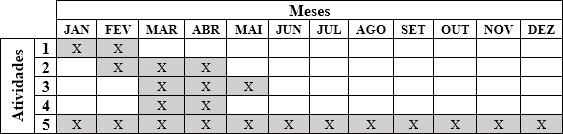
\includegraphics[scale=1]{imagens/cronograma}
\end{figure*}
\FloatBarrier

\begin{enumerate}
	\item Descrição da atividade 1;
	\item Descrição da atividade 2;
	\item Descrição da atividade 3;
	\item Descrição da atividade 4;
	\item Descrição da atividade 5.
\end{enumerate}

\chapter{Conclusões e Recomendações}
\label{cap:05}

São   descritas   claramente   as   conclusões retiradas   das discussões  e  dos  experimentos  realizados  no  decorrer  da  pesquisa,  e  finalizada  a parte  textual  do  trabalho.  Recomendações  são  declarações  concisas  de  ações, julgadas necessárias a partir das conclusões obtidas, a serem usadas no futuro.


% ---
% Inserir um percentual % na frente para que não apareça na versão final
\chapter{Exemplos}
\label{cap:99}

Texto considerando a revisão da literatura pertinente, dividido em seções e subseções.

Este é um exemplo de como usar figuras. Referência cruzada: Figura~\ref{fig:exemplo}

\FloatBarrier
\begin{figure}[!htbp]
	\centering
	\caption{Exemplo de figura}
	%scale redimensiona a figura.
	%1.5 = 150% do tamanho original
	%1 = 100% do tamanho original
	%0.20 = 20% do tamanho original
	\fbox{
\includegraphics[scale=1]{imagens/IFSP-BRA.png}}
	\legend{Fonte: Disponível em: http://bra.ifsp.edu.br. Acesso em: 27 mar. 2020}
        %\legend{Fonte: Autor (ano) ou \citetext{chave}}
	\label{fig:exemplo}
\end{figure}
\FloatBarrier


Este é um exemplo de como usar tabelas. Referência cruzada: Tabela~\ref{tab:exemplo}

\FloatBarrier
\begin{table}[!htbp]
\centering
\caption{Exemplo de tabela de 2 colunas}
	\begin{tabular}{ c | c }
		\hline
		\textbf{Coluna 1} & \textbf{Coluna 2} \\ \hline
		Dado 1a           & Dado 2a           \\ \hline
		Dado 1b           & Dado 2b           \\ \hline
		Dado 1c           & Dado 2c           \\ \hline
		Dado 1d           & Dado 2d           \\ \hline
	\end{tabular}
	\\ \vspace{0.2cm}
	Fonte: Autoria própria (ano)
	\label{tab:exemplo}
\end{table}
\FloatBarrier


Este é um exemplo de como usar quadros. Referência cruzada: Quadro~\ref{qua:exemplo}

\FloatBarrier
\begin{quadro}[!htbp]
	\centering
	\caption{Exemplo de quadro}
	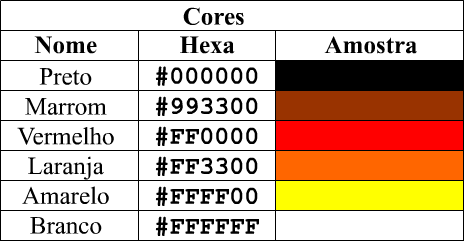
\includegraphics[scale=.7]{imagens/exemploQuadro}
	\\Fonte: Autoria própria (ano)
	\label{qua:exemplo}
\end{quadro}
\FloatBarrier

Este é um exemplo de como usar quadros. Referência cruzada: Quadro~\ref{tab:exemploquad}

\FloatBarrier
\begin{quadro}[!htbp]
\centering
\caption{Exemplo de Quadro de 3 colunas}
	\begin{tabular}{ | m{10em} | m{4cm}| m{4cm} | }
		\hline
		\textbf{Coluna 1} & \textbf{Coluna 2} & \textbf{Coluna 3} \\ \hline
		Dado 1a           & Dado 2a & \\ \hline
		Dado 1b           & Dado 2b & \\ \hline
		Dado 1c           & Dado 2c & \\ \hline
		Dado 1d           & Dado 2d & \\ \hline
	\end{tabular}
	\\ \vspace{0.2cm}
	Fonte: Autoria própria (ano)
	\label{tab:exemploquad}
\end{quadro}
\FloatBarrier

Este é um exemplo de como usar quadros. Referência cruzada: Quadro~\ref{tab:exemplo2}

\FloatBarrier
\begin{quadro}[!htbp]
\centering
\caption{Exemplo de Quadro de 2 colunas}
	\begin{tabular}{ | m{10em} | m{4cm}| }
		\hline
		\textbf{Coluna 1} & \textbf{Coluna 2}  \\ \hline
		Dado 1a           & Dado 2a  \\ \hline
		Dado 1b           & Dado 2b  \\ \hline
		Dado 1c           & Dado 2c  \\ \hline
		Dado 1d           & Dado 2d  \\ \hline
	\end{tabular}
	\\ \vspace{0.2cm}
	Fonte: Autoria própria (ano)
	\label{tab:exemplo2}
\end{quadro}
\FloatBarrier

Este é um exemplo de como usar equações. Referência cruzada: Equação~\ref{eq:exemplo}

\begin{equation}
\sum_{i=1}^{n} i = \frac{n(n+1)}{2}
\label{eq:exemplo}
\end{equation}

\clearpage

Exemplo de inserção de lista de código fonte (\textbf{\textcolor{red}{não use acentos no código!}}):

\lstinputlisting[language=Java]{fontes/ClasseExemplo.java} 



Este é um exemplo de como inserir texto sem formatação (ambiente verbatim):

\begin{verbatim}
	Texto sem formatação, como espaçamento igual.
\end{verbatim}


Exemplo de lista de itens:

\begin{itemize}
	\item \textbf{Item 1:} texto...;
	\item \textbf{Item 2:} texto...;
    \begin{itemize}
            \item \textbf{Subitem:} texto...;
            \item \textbf{Subitem:} texto...;
            \item \textbf{Subitem:} texto...;
        \end{itemize}
	\item \textbf{Item 3:} texto...;
	\item \textbf{Item n:} texto....
\end{itemize}


Exemplo de lista numerada:

\begin{enumerate}
	\item \textbf{Item:} texto...;
	\item \textbf{Item:} texto...;
    \begin{enumerate}
        \item \textbf{Subitem:} texto...;
        \item \textbf{Subitem:} texto...;
        \item \textbf{Subitem:} texto...;
    \end{enumerate}
	\item \textbf{Item:} texto...;
	\item \textbf{Item:} texto....
\end{enumerate}

Tipos de referência a serem utilizados no arquivo referencias.bib:
Exemplos de estruturas.\\

@article{<citation key>,
    author        = {},
    title         = {},
    journaltitle  = {},
    year          = {}
}

@online{<citation key>,
    author        = {},
    title         = {},
    year          = {},
    url           = {},
    urlaccessdate = {}
}

@book{<citation key>,
    author        = {},
    title         = {},
    year          = {}
}

@misc{<citation key>,
    author        = {},
    title         = {},
    year          = {},
    url           = {},
    urlaccessdate = {}
}


Exemplos de comandos para texto e referências:

\begin{itemize}
	\item Para iniciar um novo parágrafo, basta deixar uma linha em branco no código fonte;
	\item Não force o compilador a pular mais de uma linha, pois terá influência negativa na composição do documento;
	\item Sempre deixe o \LaTeX\ realizar a formatação de parágrafos e posicionamento de elementos;
	\item Utilização de aspas simples (abertura \verb|`|, fechamento \verb|'|): `Texto entre aspas simples';
	\item Utilização de aspas duplas (abertura \verb|``|, fechamento \verb|''|): ``Texto entre aspas duplas'';
	\item Negrito (comando \verb|\textbf|): \textbf{texto em negrito};
	\item Itálico (comando \verb|\textit|): \textit{texto em itálico};
	\item Sublinhado (comando \verb|\underline|): \underline{texto sublinhado};
	\item Negrito e itálico (usar comandos juntos): \textbf{\textit{texto em negrito e itálico}};
	\item Alterar cor do texto (comando \verb|\textcolor{cor}{texto}|):
	\begin{itemize}
		\item Exemplo \verb|\textcolor{red}{texto}|: \textcolor{red}{texto vermelho};
		\item Exemplo \verb|\textcolor[RGB]{255, 102, 0}|: \textcolor[RGB]{255, 102, 0}{texto laranja};
		\item Exemplo \verb|\textcolor[HTML]{006AD7}|: \textcolor[HTML]{006AD7}{texto azul};
	\end{itemize}
	\item Ambiente matemático inline (comando \verb|$ expressão $|): $s = x^2-2x +1$;
	\item Referência normal (comando \verb|\cite|):
	\begin{itemize}
		\item \cite{Agaisse1995};
		\item \cite{Abedi2014};
		\item \cite{Baum2016};
        
	\end{itemize}
	\item Referência normal com mais de uma obra (comando \verb|\cite|):
	\begin{itemize}
		\item \cite{Abedi2014, Agaisse1995};
		\item \cite{AgapitoTenfen2014, Baum2016, Nelson2014};
	\end{itemize}
	\item Referência nome e ano (comando \verb|\citeauthorandyear|):
	\begin{itemize}
		\item \citeauthorandyear{bervian2007a};
		\item \citeonline{bervian2007a};
		\item \citeauthorandyear{documento2018};
		\item \citeauthorandyear{Abedi2014};
        \item \citeonline{schaefer2022};
        \item \citeonline{castro2019};
	\end{itemize}
	\item Referência apud ({mais antigo} {mais novo}):\\
	\verb|\apud[pagina]{autor-indireto}{autor-direto}|):
	\begin{itemize}
		\item \apud{Agaisse1995}{Abedi2014};
		\item \apudonline{Agaisse1995}{Abedi2014};
	\end{itemize}
	\item Referência apud [pagina]({mais antigo} {mais novo}):\\
	\verb|\apud[pagina]{autor-indireto}{autor-direto}|):
	\begin{itemize}
		\item \apud[p. 81]{Agaisse1995}{Abedi2014};
		\item \apudonline[p. 81]{Agaisse1995}{Abedi2014};
	\end{itemize}
	
	\item Referência do mesmo autor, mesmo ano com obras distintas 
	\verb|\citeauthorandyear|):
	\begin{itemize}
		\item \citeauthorandyear{Agaisse1996a};
		\item \citeauthorandyear{Agaisse1996b};
		\item \cite{Agaisse1996a};
		\item \cite{Agaisse1996b};
	\end{itemize}
	
	
\end{itemize}


Exemplo 1 de citação direta:

\begin{citacao}
	Os 20 aminoácidos usualmente encontrados como resíduos em proteínas contém um grupo $\alpha$-carboxil, um grupo $\alpha$-amino e um grupo R distinto substituído no átomo de carbono $\alpha$. O átomo de carbono $\alpha$ de todos os aminoácidos, com exceção da glicina, é assimétrico e, portanto, os aminoácidos podem existir em pelo menos duas formas estereoisoméricas. Somente os estereoisômeros L, com uma configuração relacionada à configuração absoluta da molécula de referência L-gliceraldeído, são encontrados em proteínas \cite[p. 81]{Nelson2014}.
\end{citacao}

Exemplo 2 de citação direta:

\begin{citacao}
	\textit{These various insecticidal proteins are synthesized during the stationary phase and accumulate in the mother cell as a crystal inclusion which can account for up to 25\% of the dry weight of the sporulated cells. The amount of crystal protein produced by a B. thuringiensis culture in laboratory conditions (about 0.5 mg of protein per ml) and the size of the crystals (24) indicate that each cell has to synthesize $10^6$ to $2 \times 10^6$ $\delta$-endotoxin molecules during the stationary phase to form a crystal} \cite[p. 1]{Agaisse1995}.
\end{citacao}

Exemplo de nota de rodapé\footnote{Essa é uma nota de rodapé!}.

Exemplo de rodapé com referência indicada nele\footnote{\citetext{marciano2020}}

% ---




% ----------------------------------------------------------
% Referências bibliográficas
% ----------------------------------------------------------
\postextual
\bibliography{referencias}

\end{document}
